\documentclass[conference]{IEEEtran}
\IEEEoverridecommandlockouts
\usepackage{cite}
\usepackage{amsmath,amssymb,amsfonts}
\usepackage{graphicx}
\usepackage{textcomp}
\usepackage{xcolor}
\usepackage{booktabs}
\usepackage{url}

\graphicspath{{../figures/}}

% Every measured number is a double-brace placeholder, filled from
% results/numbers.json by scripts/fill_numbers.py. The keys are listed in
% deliverables/NUMBER_KEYS.md. Compile the filled copy, not this source.
% The pct style prints a bare percent sign, which LaTeX reads as a comment,
% so this file never uses it.

\begin{document}

\title{Which File Gave It Away? Shortcut-Neutral Evaluation of Audio-Visual
Deepfake Detection with a Real-Only Lip-Sync Detector}

\author{\IEEEauthorblockN{Vaibhav Shiroorkar}
\IEEEauthorblockA{\textit{Dept. of Electronics and Computer Engineering} \\
\textit{KJ Somaiya School of Engineering}\\
Mumbai, India \\
v.shiroorkar@somaiya.edu}
\and
\IEEEauthorblockN{Adithya Jithesh}
\IEEEauthorblockA{\textit{Dept. of Electronics and Computer Engineering} \\
\textit{KJ Somaiya School of Engineering}\\
Mumbai, India \\
adithya.j@somaiya.edu}
\and
\IEEEauthorblockN{Shivansh Gupta}
\IEEEauthorblockA{\textit{Dept. of Electronics and Computer Engineering} \\
\textit{KJ Somaiya School of Engineering}\\
Mumbai, India \\
shivansh.gupta@somaiya.edu}
\and
\IEEEauthorblockN{Tejashree Phatak}
\IEEEauthorblockA{\textit{Dept. of Electronics and Computer Engineering} \\
\textit{KJ Somaiya School of Engineering}\\
Mumbai, India \\
tejashree@somaiya.edu}
}

\maketitle

\begin{abstract}
Audio-visual deepfake detectors score close to perfect on their own
benchmarks and fail on clips from elsewhere. We show that part of that
benchmark accuracy comes from how the files were made. A classifier that reads
only file metadata and audio edges predicts the FakeAVCeleb label at
{{audit.fakeavceleb.raw.clip}} AUC and the HiFi-AVDF label at
{{audit.hifiavdf.raw.clip}}: codecs, lengths and frame sizes follow the
label. We remove these cues with one codec, a fixed 3.00~s span from the first
sound, one loudness level, and dither. This lowers the FakeAVCeleb ceiling to
{{audit.fakeavceleb.neutral.clip}}, which
misses our preregistered bar of 0.60. We then train a lip-sync detector on real clips only, with frozen AV-HuBERT features. Its test
AUC is {{sync.test.seed17.auc}}, {{sync.test.seed29.auc}} and
{{sync.test.seed43.auc}} over three seeds. Its scores follow the mechanism:
voice cloning is caught best, and face swaps that keep the original lips
least. On three corpora it never saw, its AUC falls to between
{{sync.dfdc.seed17.auc}} and {{sync.lavdf-window.seed29.auc}}. A threshold
set from 200 real clips of a new corpus flags {{h4.hifiavdf-seed43.conformal_real_only.fpr}}
to {{h4.hifiavdf-seed17.conformal_real_only.fpr}} of real HiFi-AVDF clips,
against {{h4.hifiavdf-seed43.source_validation.fpr}} to
{{h4.hifiavdf-seed17.source_validation.fpr}} with the training threshold, but
then catches few fakes. Late fusion of the visual, audio and sync paths
changes AUC over the visual path alone by {{h2.dfdc.estimate}} on DFDC and {{h2.lavdf-window.estimate}} on
LAV-DF, and passes its preregistered rule. But the LAV-DF gain is over a
visual path that ranks fakes below chance, and the FakeAVCeleb gain comes only
from cloned-voice clips the visual path cannot see.
\end{abstract}

\begin{IEEEkeywords}
Audio-visual deepfakes, shortcut learning, dataset audit, lip-sync detection,
false-alarm control, preregistration.
\end{IEEEkeywords}

\section{Introduction}

Audio-visual deepfake detectors report near-perfect AUC on the corpus they
were trained on. On clips from another source they often fall toward chance.
A common reading is that the detectors overfit to one generator. We test a
simpler reading: the benchmark files themselves carry the label.

Every fake in a dataset passes through a production pipeline. A voice cloning
tool writes its own audio format. A face-swap tool writes its own video codec.
A text-to-speech system pads its output with digital silence. Real clips pass
through a different pipeline. A detector can learn these file habits instead
of the manipulation, and its benchmark score will not tell us which it learned.

We measure this directly. A gradient-boosted model that never sees a pixel or
hears a word predicts the FakeAVCeleb~\cite{fakeavceleb} label at
{{audit.fakeavceleb.raw.clip}} AUC. It reads only codec, bitrate, frame size,
duration, and the silence at each end of the audio track. On HiFi-AVDF, a
recent corpus built with six commercial video generators~\cite{havic}, the
same model reaches {{audit.hifiavdf.raw.clip}}. A detector score on either
corpus means little until it is compared with that ceiling.

We make five contributions:

\begin{enumerate}
\item \textit{A shortcut census.} We audit FakeAVCeleb, LAV-DF~\cite{lavdf},
DFDC~\cite{dfdc} and HiFi-AVDF with cue-only classifiers. We report the
ceiling each corpus allows from file cues alone, a per-category codec census
for FakeAVCeleb, and per-generator file fingerprints for HiFi-AVDF.
\item \textit{A shortcut-neutral protocol.} Every clip gets one codec, a fixed
3.00~s span from the first sound, a fixed loudness and dither. We show that
naive cleaning fails, explain why, and report the residual cue and the clips
that cleaning removes.
\item \textit{A lip-sync detector trained on real clips only.} It never sees a
fake, so it cannot learn a generator's habits. Its scores per manipulation
method follow what each method does to the lips and the voice.
\item \textit{False-alarm control from real clips only.} We compare a
threshold calibrated on real clips from the new domain with the threshold
carried over from training.
\item \textit{A preregistered fusion test.} We fuse visual, audio and sync
paths with a model fixed before any branch was trained, and test it against
the visual path alone on three locked corpora.
\end{enumerate}

We do not claim a new architecture. Our hypotheses were committed before the
runs, and we report the one that failed.

\section{Related Work}

\textit{Audio-visual detectors.} AVFF~\cite{avff} fuses audio and visual
features after audio-visual pretraining on real speech and reports cross-corpus
results, with no control for file cues. AVH-Align~\cite{smeu2025} trains an
alignment model on frozen AV-HuBERT~\cite{avhubert} features using real clips
only, and shows that it keeps its score when the leading silence is trimmed.
HAVIC~\cite{havic} fine-tunes on FakeAVCeleb and introduces HiFi-AVDF. These
works, like most in the area, split FakeAVCeleb at random rather than by
person. Our sync detector follows the real-only idea of AVH-Align, and we do
not claim that idea. What we add is a measurement of such a detector under a
protocol that removes file cues from both training and test data, with
identity-grouped splits and a breakdown by manipulation method. Fusion of
several modalities is not new either. We test it only as a preregistered
comparison with the visual path under the same shortcut control.

\textit{Dataset shortcuts.} M\"uller et al.~\cite{muller2021} showed that
silence duration alone separates real and spoofed speech in ASVspoof 2019 LA.
Smeu et al.~\cite{smeu2025} found leading digital silence in FakeAVCeleb and
AV-Deepfake1M, flagged trailing silence, and trimmed it at test time only.
DeepFake Doctor~\cite{deepfakedoctor} confirmed the silence cue, showed that
FakeAVCeleb's leave-one-out protocol leaks Wav2Lip content, and proposed an
identity split and temporal jittering. For generated images, Grommelt et
al.~\cite{grommelt} showed that JPEG compression and image size follow the
label. Pagon et al.~\cite{pagon2026} ask what deepfake benchmarks measure,
with linear probes on frozen self-supervised features. They audit video,
image and audio benchmarks, but no audio-visual corpus and no file cues.
DFD-Lab~\cite{dfdlab2026} trains three audio-visual detectors on
FakeAVCeleb and reports AUROC near 0.5 on a filtered Deepfake-Eval-2024
subset, with no shortcut control.
We found no published per-category codec census for an audio-visual deepfake
corpus, no classifier trained on container metadata alone, and no
neutralization applied to training and test data that covers codec, both
silence edges, loudness and length together. The silence cue itself is theirs.
The codec census, the joint neutralization and the HiFi-AVDF audit are ours.

\textit{Modality prediction.} Multimodaltrace~\cite{multimodaltrace} trains a
multi-label head on FakeAVCeleb. Yu et al.~\cite{yu2023} train a dual-label
classifier and report per-modality accuracy across DFDC and FakeAVCeleb.
MRDF~\cite{mrdf} uses per-modality labels as regularizers and argues that
clip-level labels harm fused learning, with in-dataset evidence. A
per-modality head is therefore not new. Our preregistration includes a test of
whether such predictions transfer between FakeAVCeleb and LAV-DF under
shortcut control. Only one direction has run (Section~\ref{sec:overnight}).

\textit{False-alarm control.} Split conformal p-values on an inlier reference
set~\cite{bates2023} and the Neyman-Pearson umbrella
algorithm~\cite{tong2018} give standard false-positive guarantees from
negative examples alone. Recent work already shows that detector thresholds
fail to transfer across domains even when AUC holds~\cite{nguyen2026,
laionmobile}, so we do not present that as a finding. Two concurrent records
are close to our test. Mahdaoui~\cite{mahdaoui2026} preregisters real-photo
recalibration of still-image detectors under camera-processing shift.
PGA-G~\cite{pgag2026} sets conformal operating points from genuine speech. We
claim neither the method nor the general idea. Our test applies it to an
audio-visual video detector moved across corpora, calibrated on real target
clips only.

\section{Shortcut Audit}

\subsection{Method}

The audit reads each clip's container and stream metadata and the edges of its
audio track, and nothing else. The cues are video and audio codec, video and
audio bitrate, frame size, frame rate, audio sample rate, duration, leading
and trailing digital silence, and loudness. We score two things. A single-cue
AUC measures how well one cue alone separates the classes. The shortcut
ceiling is the out-of-fold AUC of gradient-boosted trees given all cues, over
five folds grouped by identity. HiFi-AVDF folds are grouped by real-generated
pair, and LAV-DF is audited per file, because a window manifest lets one file
supply both labels. We report the ceiling for three labels: the clip label,
video-fake and audio-fake. A higher ceiling means a weaker benchmark: a
detector on that corpus should be compared with it, not with 0.5.

We audit all of FakeAVCeleb, a stratified sample of
{{audit.lavdf.raw.clips|int}} LAV-DF files, a
{{audit.dfdc.raw.clips|int}}-clip subset of DFDC, and all
{{audit.hifiavdf.raw.clips|int}} HiFi-AVDF clips. The DFDC subset contains no
fake audio, so it has no audio-label ceiling.

\subsection{Ceilings}

\begin{table}[htbp]
\caption{Shortcut ceiling (ROC-AUC) from file and audio-edge cues alone}
\label{tab:ceiling}
\centering
\begin{tabular}{lrrrr}
\toprule
 & \multicolumn{3}{c}{Raw files} & Neutral \\
\cmidrule(lr){2-4}
Corpus & Clip & Video & Audio & Clip \\
\midrule
FakeAVCeleb & {{audit.fakeavceleb.raw.clip}} & {{audit.fakeavceleb.raw.video}} & {{audit.fakeavceleb.raw.audio}} & {{audit.fakeavceleb.neutral.clip}} \\
LAV-DF & {{audit.lavdf.raw.clip}} & {{audit.lavdf.raw.video}} & {{audit.lavdf.raw.audio}} & {{audit.lavdf.neutral.clip}} \\
DFDC & {{audit.dfdc.raw.clip}} & {{audit.dfdc.raw.video}} & n/a & {{audit.dfdc.neutral.clip}} \\
HiFi-AVDF & {{audit.hifiavdf.raw.clip}} & {{audit.hifiavdf.raw.video}} & {{audit.hifiavdf.raw.audio}} & {{audit.hifiavdf.neutral.clip}} \\
\bottomrule
\end{tabular}
\end{table}

Table~\ref{tab:ceiling} gives the ceilings. FakeAVCeleb's labels can be read
from its files. LAV-DF is different. Every one of its categories is H.264 with
AAC audio, so the codec carries nothing. But weak cues add up: audio bitrate,
trailing silence and duration together give the ceiling in the table.
Neutralization can fix the bitrate and the silence. It cannot fix duration on
whole files, because LAV-DF's edits replace words and change a file's length.
Our detector reads fixed windows and never sees that length, but a model given
whole files could learn it.

DFDC is close to clean on these cues. This may be one reason detectors trained
on FakeAVCeleb fall toward chance on DFDC: the cue they learned is absent. The
neutral ceilings for LAV-DF, DFDC and HiFi-AVDF come from the same audit run
on their neutral copies.

\subsection{FakeAVCeleb codec census}

\begin{table*}[htbp]
\caption{FakeAVCeleb clips per category: codecs in the raw files, and clips
kept after neutralization}
\label{tab:census}
\centering
\begin{tabular}{lrllr}
\toprule
Category & Raw clips & Video codec & Audio codec & Kept \\
\midrule
Real video, real audio & {{audit.fakeavceleb.raw.census.RealVideo-RealAudio.clips|int}} & H.264 (all) & AAC (all) & {{audit.fakeavceleb.neutral.census.RealVideo-RealAudio.clips|int}} \\
Real video, fake audio & {{audit.fakeavceleb.raw.census.RealVideo-FakeAudio.clips|int}} & H.264 (all) & MP3 ({{audit.fakeavceleb.raw.census.RealVideo-FakeAudio.audio_codec.mp3|int}}), AAC ({{audit.fakeavceleb.raw.census.RealVideo-FakeAudio.audio_codec.aac|int}}) & {{audit.fakeavceleb.neutral.census.RealVideo-FakeAudio.clips|int}} \\
Fake video, real audio & {{audit.fakeavceleb.raw.census.FakeVideo-RealAudio.clips|int}} & MPEG-4 ({{audit.fakeavceleb.raw.census.FakeVideo-RealAudio.video_codec.mpeg4|int}}), H.264 ({{audit.fakeavceleb.raw.census.FakeVideo-RealAudio.video_codec.h264|int}}) & AAC (all) & {{audit.fakeavceleb.neutral.census.FakeVideo-RealAudio.clips|int}} \\
Fake video, fake audio & {{audit.fakeavceleb.raw.census.FakeVideo-FakeAudio.clips|int}} & MPEG-4 (all) & AAC (all) & {{audit.fakeavceleb.neutral.census.FakeVideo-FakeAudio.clips|int}} \\
\bottomrule
\end{tabular}
\end{table*}

Table~\ref{tab:census} shows the census. Every real clip is H.264 with AAC
audio. Generated speech in the real-video category is stored almost entirely
as MP3. Most face-swapped clips, and every clip with both streams faked, are
MPEG-4 Part~2. A detector that learns ``MPEG-4 means fake'' or ``MP3 means
fake'' needs no face and no voice. Clips with generated audio also start and
end with digital silence, while real clips start with noise. To our knowledge,
neither the MP3 track nor the per-category codec split has been reported for
this corpus.

\subsection{HiFi-AVDF generator fingerprints}

HiFi-AVDF pairs each real video with a copy made by one of six commercial
generators: Kling~2.5, PixVerse~V5, Seedance~1.0, Sora~2, Veo~3.1 and
Wan~2.5. Each generator leaves its own mark in the file. Real clips share one
frame size, and five of the six generators write a different one. Sora~2 and
Veo~3.1 write every clip at one fixed length, while real clip lengths vary.
Seedance writes at a much higher bitrate than the real clips. Kling and
Seedance clips start with digital silence, and real clips do not. None of
these cues needs the content of the video. Together they give the
{{audit.hifiavdf.raw.clip}} ceiling in Table~\ref{tab:ceiling}. Any score on
the raw files has to be read against it.

\section{Shortcut-Neutral Protocol}

\begin{figure}[htbp]
\centerline{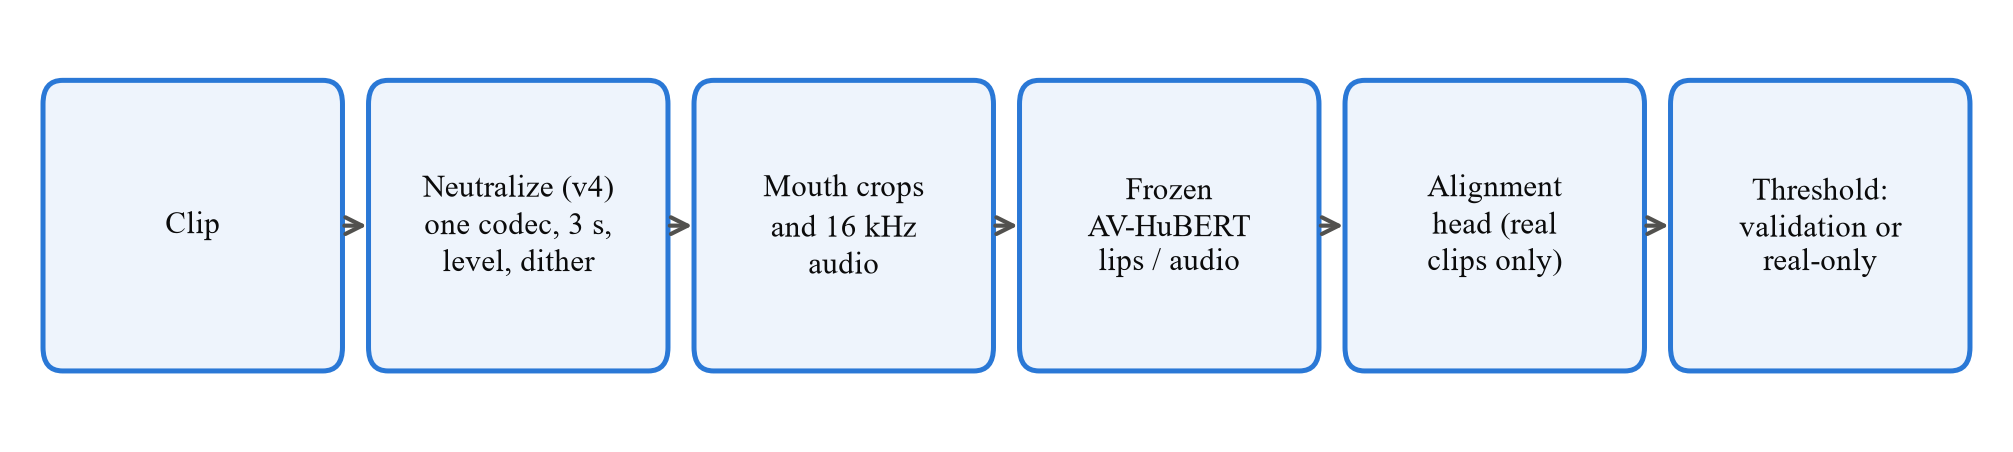
\includegraphics[width=\columnwidth]{fig_pipeline.png}}
\caption{The pipeline. Each clip is neutralized, cut into two lip and audio
windows, and scored by a frozen AV-HuBERT encoder and an alignment head
trained on real clips only. The threshold comes from source validation or
from real target clips.}
\label{fig:pipeline}
\end{figure}

\subsection{Why the first neutralizer failed}

Our first neutralizer cut each clip with an ffmpeg input seek, normalized
loudness with a standard filter, and re-encoded both streams. It looked
correct. The audit said otherwise (Table~\ref{tab:h1}). AAC encoders add a
short run of priming samples at the start of a stream. Re-muxing exposed each
source's priming differently, so face-swapped clips gained leading silence
that real clips did not. Duration and trailing silence also still differed by
class. Cleaning had put the shortcut back.

\begin{table}[htbp]
\caption{H1: shortcut ceiling (ROC-AUC) on neutral FakeAVCeleb copies; the
preregistered bar is 0.60 on the clip label}
\label{tab:h1}
\centering
\begin{tabular}{lrrrr}
\toprule
Attempt & Clips & Clip & Video & Audio \\
\midrule
1, neutralizer v1 & {{audit.fakeavceleb.v1.clips|int}} & {{audit.fakeavceleb.v1.clip}} & {{audit.fakeavceleb.v1.video}} & {{audit.fakeavceleb.v1.audio}} \\
check, v4 sample & {{audit.fakeavceleb.v4check.clips|int}} & {{audit.fakeavceleb.v4check.clip}} & {{audit.fakeavceleb.v4check.video}} & {{audit.fakeavceleb.v4check.audio}} \\
2, neutralizer v4 & {{audit.fakeavceleb.neutral.clips|int}} & {{audit.fakeavceleb.neutral.clip}} & {{audit.fakeavceleb.neutral.video}} & {{audit.fakeavceleb.neutral.audio}} \\
\bottomrule
\end{tabular}
\end{table}

\subsection{Neutralizer v4}

Version 4 never lets ffmpeg touch the audio timeline before encoding. For
every clip it does the following:

\begin{enumerate}
\item Decode the audio once to 16~kHz mono samples.
\item Scale the samples to $-23$~dBFS RMS with a plain gain in numpy, so no
filter can add a clip-dependent delay.
\item Find the first sample above $-60$~dBFS. Round that start up to a whole
video frame and keep exactly 3.00~s from there. Refuse the clip if it has less
than 3.00~s of sound.
\item Add dither at $-66$~dBFS. Speech synthesizers write exact digital zeros
in their pauses, and microphones never do.
\item Re-encode the video for that span as H.264 at 25~fps with one constant
quality setting, mux the audio as AAC, and strip container metadata.
\end{enumerate}

Fixing the length removes duration as a cue. Starting at the first sound
removes leading silence. HiFi-AVDF also gets one frame size, the native size
of its real clips, because frame size follows its labels. We first checked
version 4 on a sample of 150 clips per category that is used for nothing else.
The check row of Table~\ref{tab:h1} counts the clips it kept.

\subsection{H1 result}

Our preregistered test H1 required the clip-label ceiling on neutral
FakeAVCeleb to be at most 0.60. Version 4 gives
{{audit.fakeavceleb.neutral.clip}} on {{audit.fakeavceleb.neutral.clips|int}}
clips. \textbf{H1 is not met.} The strongest remaining single cue is video
bitrate. Every clip is encoded at the same constant quality, so bitrate
follows image content: smoother face swaps compress into fewer bits. That
makes it a property of the manipulated pixels rather than of a generator's
file pipeline. But H1 was defined on all cues, so it fails as written. The
audio label keeps a higher ceiling, {{audit.fakeavceleb.neutral.audio}},
mainly from small differences at the clip edges and from loudness after AAC
encoding.

\subsection{What cleaning removes}

Version 4 refuses {{neutral.fakeavceleb.refused|int}} FakeAVCeleb clips as too
short. Every refused clip carries generated speech, and no real clip is
refused (Table~\ref{tab:census}, last column). This is a selection effect.
Generated speech is shorter than real speech, so the neutral test set keeps
fewer fakes, and the fakes it keeps are the longer ones. We report it beside
every result on these copies.

\subsection{Preregistration and receipts}

We committed the hypotheses, success bars, seeds and splits (P-001) before any
model was trained on neutral data. Changes are dated amendments, each
committed before the run it affects. Every evaluation writes a receipt with
its command and the hashes of its inputs, code and outputs.

\section{Real-Only Sync Detector}

\subsection{Method}

The sync path asks whether the lips match the sound. We crop 88-pixel grey
mouth images at 25~fps from face landmarks. A frozen AV-HuBERT Base
encoder~\cite{avhubert} encodes the lips and the audio in two separate
passes, one with each modality alone. Each neutral clip gives two 2~s
windows, starting at 0~s and 1~s.

A small alignment head takes a lips frame and an audio frame and predicts
whether they belong together. Its input is both feature vectors, their
product and their absolute difference. Positive pairs are aligned frames of a
real clip. Negative pairs are the same lips with audio from another time or
from another clip. The head trains and selects its epoch on real clips only,
so it never sees a fake. A window's score is its mean misfit,
$-\log\sigma(g)$ over aligned frame pairs, where $g$ is the head's logit. A
clip's score is the mean over its windows.

We split FakeAVCeleb 70/15/15 by source identity. Its identity graph is fully
connected, because every person also appears as the target of someone else's
swap. We therefore also report an identity-strict test subset, whose people
never appear in training. We train at seeds 17, 29 and 43. Intervals are 95\%
from 1,000 bootstrap resamples of people, not clips. The source threshold
maximizes balanced accuracy on validation, which does contain fakes. The file
that holds it records the clips it was chosen on.

\subsection{In-domain results}

\begin{table}[htbp]
\caption{Sync path on neutral FakeAVCeleb (ROC-AUC, 95\% identity-bootstrap
interval); FPR and balanced accuracy at the validation threshold}
\label{tab:sync}
\centering
\begin{tabular}{llrr}
\toprule
Seed & ROC-AUC & FPR & Bal. acc. \\
\midrule
\multicolumn{4}{l}{\textit{Test, {{sync.test.seed17.n|int}} clips}} \\
17 & {{sync.test.seed17.auc}} [{{sync.test.seed17.auc_low}}, {{sync.test.seed17.auc_high}}] & {{sync.test.seed17.fpr}} & {{sync.test.seed17.balanced_accuracy}} \\
29 & {{sync.test.seed29.auc}} [{{sync.test.seed29.auc_low}}, {{sync.test.seed29.auc_high}}] & {{sync.test.seed29.fpr}} & {{sync.test.seed29.balanced_accuracy}} \\
43 & {{sync.test.seed43.auc}} [{{sync.test.seed43.auc_low}}, {{sync.test.seed43.auc_high}}] & {{sync.test.seed43.fpr}} & {{sync.test.seed43.balanced_accuracy}} \\
\midrule
\multicolumn{4}{l}{\textit{Identity-strict test, {{sync.test-identity-strict.seed17.n|int}} clips}} \\
17 & {{sync.test-identity-strict.seed17.auc}} [{{sync.test-identity-strict.seed17.auc_low}}, {{sync.test-identity-strict.seed17.auc_high}}] & {{sync.test-identity-strict.seed17.fpr}} & {{sync.test-identity-strict.seed17.balanced_accuracy}} \\
29 & {{sync.test-identity-strict.seed29.auc}} [{{sync.test-identity-strict.seed29.auc_low}}, {{sync.test-identity-strict.seed29.auc_high}}] & {{sync.test-identity-strict.seed29.fpr}} & {{sync.test-identity-strict.seed29.balanced_accuracy}} \\
43 & {{sync.test-identity-strict.seed43.auc}} [{{sync.test-identity-strict.seed43.auc_low}}, {{sync.test-identity-strict.seed43.auc_high}}] & {{sync.test-identity-strict.seed43.fpr}} & {{sync.test-identity-strict.seed43.balanced_accuracy}} \\
\bottomrule
\end{tabular}
\end{table}

Table~\ref{tab:sync} gives the results. On the test set the AUC is
{{sync.test.seed17.auc}}, {{sync.test.seed29.auc}} and
{{sync.test.seed43.auc}} for the three seeds. The identity-strict subset gives
the same picture. Every interval lies above the neutral shortcut ceiling of
{{audit.fakeavceleb.neutral.clip}}, so the sync path does better than file
cues alone can on the same copies. The operating point is weaker than the
ranking. At the threshold chosen on validation, the false-positive rate on
real test clips lies between {{sync.test.seed43.fpr}} and
{{sync.test.seed17.fpr}}. The identity-strict subset keeps every real test
clip, so its FPR is the same. That false-alarm rate is the problem our fourth
contribution addresses.

\subsection{Per-method results}

\begin{table}[htbp]
\caption{Sync path ROC-AUC per manipulation method, neutral FakeAVCeleb test}
\label{tab:methods}
\centering
\begin{tabular}{lrrr}
\toprule
Method & Seed 17 & Seed 29 & Seed 43 \\
\midrule
Voice cloning (RTVC) & {{sync.test.seed17.method.rtvc}} & {{sync.test.seed29.method.rtvc}} & {{sync.test.seed43.method.rtvc}} \\
Wav2Lip & {{sync.test.seed17.method.wav2lip}} & {{sync.test.seed29.method.wav2lip}} & {{sync.test.seed43.method.wav2lip}} \\
FaceSwap + Wav2Lip & {{sync.test.seed17.method.faceswap-wav2lip}} & {{sync.test.seed29.method.faceswap-wav2lip}} & {{sync.test.seed43.method.faceswap-wav2lip}} \\
FSGAN + Wav2Lip & {{sync.test.seed17.method.fsgan-wav2lip}} & {{sync.test.seed29.method.fsgan-wav2lip}} & {{sync.test.seed43.method.fsgan-wav2lip}} \\
FSGAN & {{sync.test.seed17.method.fsgan}} & {{sync.test.seed29.method.fsgan}} & {{sync.test.seed43.method.fsgan}} \\
FaceSwap & {{sync.test.seed17.method.faceswap}} & {{sync.test.seed29.method.faceswap}} & {{sync.test.seed43.method.faceswap}} \\
\bottomrule
\end{tabular}
\end{table}

Table~\ref{tab:methods} splits the test AUC by method. In all three seeds,
voice cloning scores highest, the three Wav2Lip methods come next, and the two
face swaps alone score lowest. This order matches what each method does to the
lips and the voice. Voice cloning replaces the voice and leaves the real lips, which still
move to the original words. It is caught best. Wav2Lip regenerates the lips to
fit the audio. The fit is imperfect, so it is caught well, but less well. A
face swap alone keeps the original lips and the original voice, so there is
little misalignment to find. It is caught least.

A detector that learned a generator's file habits would have no reason to
rank the methods this way. This order is evidence that the path reads lip and
audio agreement. It is not proof. The residual audio cue from H1 sits on
generated speech, which is also where voice cloning lives, so part of that
row may come from the residual cue. A direct test supports the mechanism:
moving the audio of real clips raises the misfit
(Section~\ref{sec:overnight}).

\section{Cross-Corpus and False-Alarm Results}
\label{sec:cross}

The models in this section are frozen. Nothing is retrained, selected or
thresholded on a target corpus, except the real-only calibration split that
H4 defines. Each target is audited on its raw files, neutralized with version
4, and audited again. LAV-DF is sampled by original recording, and each original comes with
all its edits, so real and fake files share speaker, room and camera.

\subsection{Cross-corpus detection}

\begin{table*}[htbp]
\caption{Sync path ROC-AUC on locked targets after neutralization (95\%
bootstrap interval), with each target's neutral shortcut ceiling}
\label{tab:cross}
\centering
\begin{tabular}{lrrrrr}
\toprule
Target & Clips & Seed 17 & Seed 29 & Seed 43 & Neutral ceiling \\
\midrule
LAV-DF test, file label & {{sync.lavdf-test.seed17.scored|int}} & {{sync.lavdf-test.seed17.auc}} [{{sync.lavdf-test.seed17.auc_low}}, {{sync.lavdf-test.seed17.auc_high}}] & {{sync.lavdf-test.seed29.auc}} [{{sync.lavdf-test.seed29.auc_low}}, {{sync.lavdf-test.seed29.auc_high}}] & {{sync.lavdf-test.seed43.auc}} [{{sync.lavdf-test.seed43.auc_low}}, {{sync.lavdf-test.seed43.auc_high}}] & {{audit.lavdf.neutral.clip}} \\
LAV-DF test, window label & {{sync.lavdf-window.seed17.scored|int}} & {{sync.lavdf-window.seed17.auc}} [{{sync.lavdf-window.seed17.auc_low}}, {{sync.lavdf-window.seed17.auc_high}}] & {{sync.lavdf-window.seed29.auc}} [{{sync.lavdf-window.seed29.auc_low}}, {{sync.lavdf-window.seed29.auc_high}}] & {{sync.lavdf-window.seed43.auc}} [{{sync.lavdf-window.seed43.auc_low}}, {{sync.lavdf-window.seed43.auc_high}}] & {{audit.lavdf.window.clip}} \\
DFDC & {{sync.dfdc.seed17.scored|int}} & {{sync.dfdc.seed17.auc}} [{{sync.dfdc.seed17.auc_low}}, {{sync.dfdc.seed17.auc_high}}] & {{sync.dfdc.seed29.auc}} [{{sync.dfdc.seed29.auc_low}}, {{sync.dfdc.seed29.auc_high}}] & {{sync.dfdc.seed43.auc}} [{{sync.dfdc.seed43.auc_low}}, {{sync.dfdc.seed43.auc_high}}] & {{audit.dfdc.neutral.clip}} \\
HiFi-AVDF & {{sync.hifiavdf.seed17.scored|int}} & {{sync.hifiavdf.seed17.auc}} [{{sync.hifiavdf.seed17.auc_low}}, {{sync.hifiavdf.seed17.auc_high}}] & {{sync.hifiavdf.seed29.auc}} [{{sync.hifiavdf.seed29.auc_low}}, {{sync.hifiavdf.seed29.auc_high}}] & {{sync.hifiavdf.seed43.auc}} [{{sync.hifiavdf.seed43.auc_low}}, {{sync.hifiavdf.seed43.auc_high}}] & {{audit.hifiavdf.neutral.clip}} \\
\bottomrule
\end{tabular}
\end{table*}

Table~\ref{tab:cross} gives the sync path's AUC on each locked target, for
each seed, beside that target's neutral shortcut ceiling. The ceiling is the
bar a score has to clear before it can be credited to content. Each target
tests something different. LAV-DF replaces single words in the audio, the
video or both, inside otherwise real recordings. Our DFDC subset has no fake audio, so every
fake there keeps its original voice. HiFi-AVDF makes whole clips with modern
commercial generators.

LAV-DF needs a second label. Our neutral copy keeps 3.00~s from the first
sound, but LAV-DF edits single words anywhere in a longer recording. In
1,307 of its 2,823 fake clips the kept window contains no edited time at all,
so under the file label those clips are real footage labelled fake. We found
this after reading the file-label results. Amendment A9 therefore adds a
window label: a clip is fake if its kept window overlaps edited time by at
least one frame. Both labels are reported. H2, which had not run, uses the
window label. Fig.~\ref{fig:cross} shows the same scores with their
intervals.

\begin{figure}[htbp]
\centerline{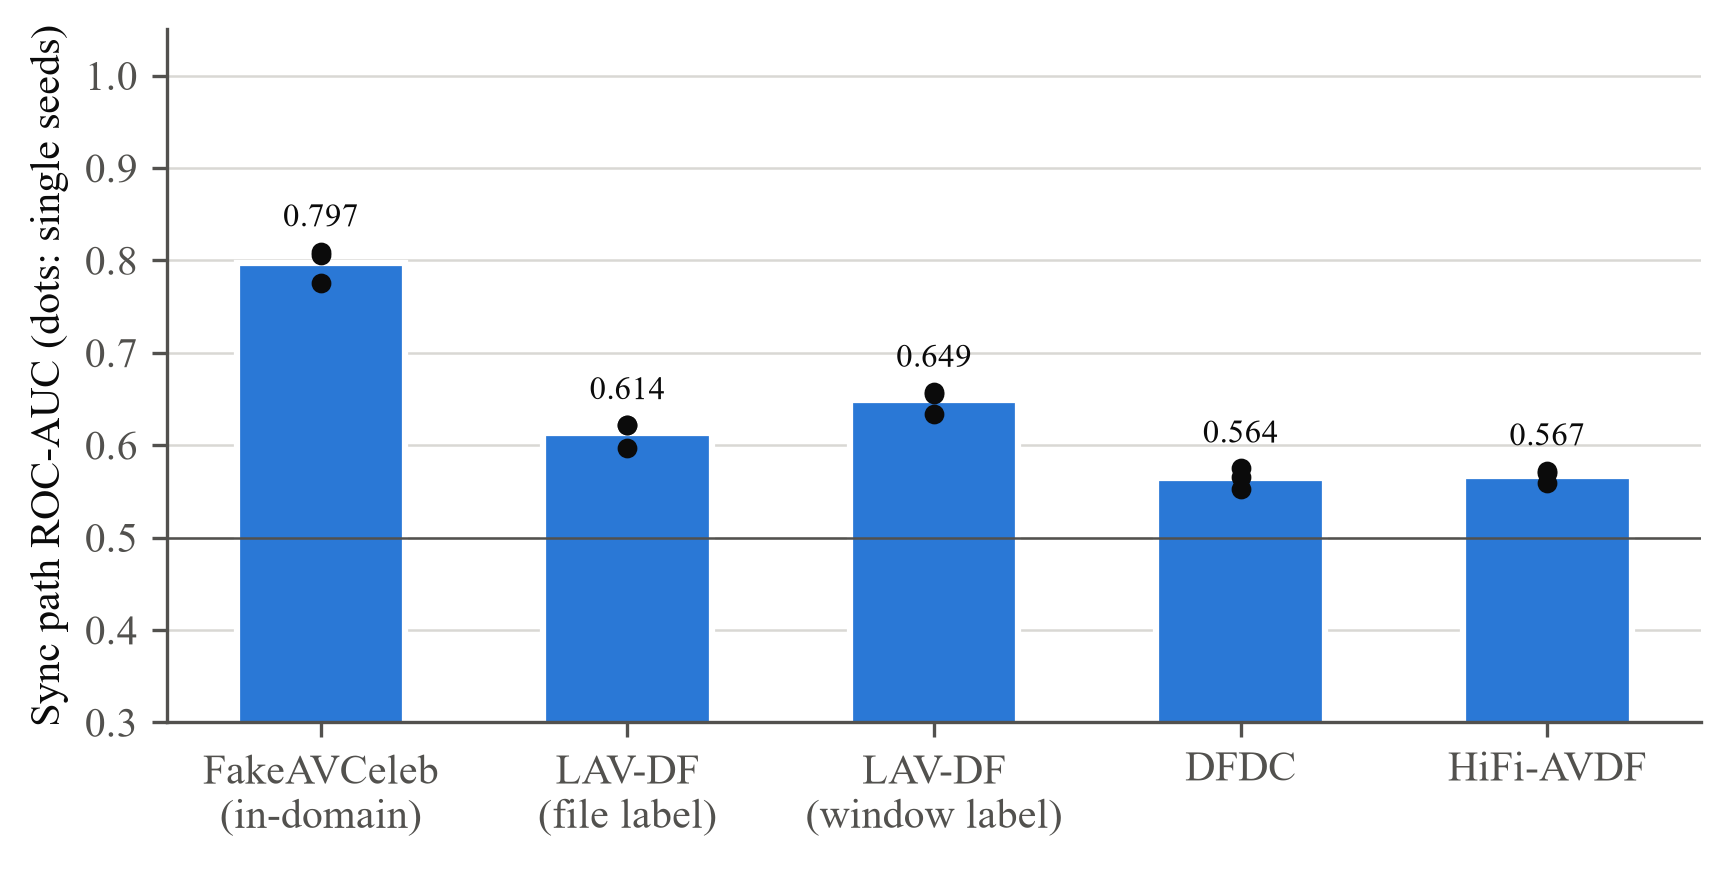
\includegraphics[width=\columnwidth]{fig_cross_corpus.png}}
\caption{Sync path ROC-AUC on the locked targets for each seed
(Table~\ref{tab:cross}).}
\label{fig:cross}
\end{figure}

\begin{table}[htbp]
\caption{Sync path ROC-AUC per generator, neutral HiFi-AVDF}
\label{tab:generators}
\centering
\begin{tabular}{lrrr}
\toprule
Generator & Seed 17 & Seed 29 & Seed 43 \\
\midrule
Kling 2.5 & {{sync.hifiavdf.seed17.method.kling2.5}} & {{sync.hifiavdf.seed29.method.kling2.5}} & {{sync.hifiavdf.seed43.method.kling2.5}} \\
PixVerse V5 & {{sync.hifiavdf.seed17.method.pixverseV5}} & {{sync.hifiavdf.seed29.method.pixverseV5}} & {{sync.hifiavdf.seed43.method.pixverseV5}} \\
Seedance 1.0 & {{sync.hifiavdf.seed17.method.seedance1.0}} & {{sync.hifiavdf.seed29.method.seedance1.0}} & {{sync.hifiavdf.seed43.method.seedance1.0}} \\
Sora 2 & {{sync.hifiavdf.seed17.method.sora2}} & {{sync.hifiavdf.seed29.method.sora2}} & {{sync.hifiavdf.seed43.method.sora2}} \\
Veo 3.1 & {{sync.hifiavdf.seed17.method.veo3.1}} & {{sync.hifiavdf.seed29.method.veo3.1}} & {{sync.hifiavdf.seed43.method.veo3.1}} \\
Wan 2.5 & {{sync.hifiavdf.seed17.method.wan2.5}} & {{sync.hifiavdf.seed29.method.wan2.5}} & {{sync.hifiavdf.seed43.method.wan2.5}} \\
\bottomrule
\end{tabular}
\end{table}

Table~\ref{tab:generators} splits HiFi-AVDF by generator. Each generator's
fakes are scored against all real clips. The raw audit showed that each
generator had its own file fingerprint. After neutralization the clips share
one codec, frame size, length and loudness, so any difference between rows
has to come from what is left in the pixels and the sound.

\textit{Reading.} The sync path keeps some signal on every target, but far
less than in its own domain. On LAV-DF it clears the neutral ceiling under
both labels. On DFDC, where every fake keeps its original voice, it sits just
above the ceiling of {{audit.dfdc.neutral.clip}}, and the seed-17 interval
includes it. On HiFi-AVDF it falls below
the neutral ceiling of {{audit.hifiavdf.neutral.clip}}: the bitrate left
after neutralization says more about the label than the lips do. The
per-generator rows explain why. PixVerse~V5 is caught best
({{sync.hifiavdf.seed17.method.pixverseV5}} at seed 17), Veo~3.1 sits near
chance ({{sync.hifiavdf.seed17.method.veo3.1}}), and Sora~2 falls below it
({{sync.hifiavdf.seed17.method.sora2}}). Generators that make sound and
picture together leave little mismatch between lips and voice, and on Sora~2
the generated clips look \emph{more} in sync than the real ones. A detector
built on lip-voice mismatch has nothing to find there.

\textit{Coverage.} The DFDC row is the result after amendment A10. The face
landmarker first found a face in only 2,110 of 6,064 DFDC windows, because
DFDC faces are small in full-HD frames, so the sync path scored 921 clips.
Locating the face with a second detector before landmarking raised this to
{{sync.dfdc.seed17.scored|int}} clips scored. AUC changed little, but the
intervals narrowed. Both versions are in the released results. HiFi-AVDF
also has {{audit.hifiavdf.raw.census.RealVideo-RealAudio.audio_codec.none|int}}
real and {{audit.hifiavdf.raw.census.FakeVideo-FakeAudio.audio_codec.none|int}}
generated source clips with no audio track, which a sync path cannot score.

\subsection{False-alarm control (H4)}

H4 asks whether a threshold set from real target clips holds the false-alarm
rate where the source threshold does not. For each target and seed, we draw
200 real target clips at random as a calibration set, with a seed fixed in
P-001. No fake label is read. Three thresholds are then scored on the
remaining target clips:

\begin{itemize}
\item \textit{Source validation:} the threshold chosen on FakeAVCeleb
validation, applied unchanged, as a deployed detector would.
\item \textit{Conformal, real only:} the split conformal
threshold~\cite{bates2023} at $\alpha = 0.05$.
\item \textit{Umbrella, real only:} the Neyman-Pearson umbrella
threshold~\cite{tong2018}, which holds the FPR at most $\alpha$ with
probability at least $1-\delta$, with $\alpha = \delta = 0.05$.
\end{itemize}

The preregistered success bar is a realized FPR of at most $\alpha + 0.02$
with the conformal threshold on every target. We do not run H4 on DFDC: our
subset has {{audit.dfdc.raw.census.RealVideo-RealAudio.clips|int}} real clips,
fewer than the 200 that calibration needs.

\begin{table*}[htbp]
\caption{H4: realized FPR and TPR on held-out target clips for each threshold
rule ($\alpha = 0.05$, 200 real calibration clips); ``Met'' is the
preregistered test on the conformal rule}
\label{tab:h4}
\centering
\begin{tabular}{llrrrrrrl}
\toprule
 & & \multicolumn{2}{c}{Source validation} & \multicolumn{2}{c}{Conformal, real only} & \multicolumn{2}{c}{Umbrella, real only} & \\
\cmidrule(lr){3-4}\cmidrule(lr){5-6}\cmidrule(lr){7-8}
Target & Seed & FPR & TPR & FPR & TPR & FPR & TPR & Met \\
\midrule
LAV-DF, file label & 17 & {{h4.lavdf-test-seed17.source_validation.fpr}} & {{h4.lavdf-test-seed17.source_validation.tpr}} & {{h4.lavdf-test-seed17.conformal_real_only.fpr}} & {{h4.lavdf-test-seed17.conformal_real_only.tpr}} & {{h4.lavdf-test-seed17.umbrella_real_only.fpr}} & {{h4.lavdf-test-seed17.umbrella_real_only.tpr}} & {{h4.lavdf-test-seed17.success}} \\
 & 29 & {{h4.lavdf-test-seed29.source_validation.fpr}} & {{h4.lavdf-test-seed29.source_validation.tpr}} & {{h4.lavdf-test-seed29.conformal_real_only.fpr}} & {{h4.lavdf-test-seed29.conformal_real_only.tpr}} & {{h4.lavdf-test-seed29.umbrella_real_only.fpr}} & {{h4.lavdf-test-seed29.umbrella_real_only.tpr}} & {{h4.lavdf-test-seed29.success}} \\
 & 43 & {{h4.lavdf-test-seed43.source_validation.fpr}} & {{h4.lavdf-test-seed43.source_validation.tpr}} & {{h4.lavdf-test-seed43.conformal_real_only.fpr}} & {{h4.lavdf-test-seed43.conformal_real_only.tpr}} & {{h4.lavdf-test-seed43.umbrella_real_only.fpr}} & {{h4.lavdf-test-seed43.umbrella_real_only.tpr}} & {{h4.lavdf-test-seed43.success}} \\
\midrule
LAV-DF, window label & 17 & {{h4.lavdf-window-seed17.source_validation.fpr}} & {{h4.lavdf-window-seed17.source_validation.tpr}} & {{h4.lavdf-window-seed17.conformal_real_only.fpr}} & {{h4.lavdf-window-seed17.conformal_real_only.tpr}} & {{h4.lavdf-window-seed17.umbrella_real_only.fpr}} & {{h4.lavdf-window-seed17.umbrella_real_only.tpr}} & {{h4.lavdf-window-seed17.success}} \\
 & 29 & {{h4.lavdf-window-seed29.source_validation.fpr}} & {{h4.lavdf-window-seed29.source_validation.tpr}} & {{h4.lavdf-window-seed29.conformal_real_only.fpr}} & {{h4.lavdf-window-seed29.conformal_real_only.tpr}} & {{h4.lavdf-window-seed29.umbrella_real_only.fpr}} & {{h4.lavdf-window-seed29.umbrella_real_only.tpr}} & {{h4.lavdf-window-seed29.success}} \\
 & 43 & {{h4.lavdf-window-seed43.source_validation.fpr}} & {{h4.lavdf-window-seed43.source_validation.tpr}} & {{h4.lavdf-window-seed43.conformal_real_only.fpr}} & {{h4.lavdf-window-seed43.conformal_real_only.tpr}} & {{h4.lavdf-window-seed43.umbrella_real_only.fpr}} & {{h4.lavdf-window-seed43.umbrella_real_only.tpr}} & {{h4.lavdf-window-seed43.success}} \\
\midrule
HiFi-AVDF & 17 & {{h4.hifiavdf-seed17.source_validation.fpr}} & {{h4.hifiavdf-seed17.source_validation.tpr}} & {{h4.hifiavdf-seed17.conformal_real_only.fpr}} & {{h4.hifiavdf-seed17.conformal_real_only.tpr}} & {{h4.hifiavdf-seed17.umbrella_real_only.fpr}} & {{h4.hifiavdf-seed17.umbrella_real_only.tpr}} & {{h4.hifiavdf-seed17.success}} \\
 & 29 & {{h4.hifiavdf-seed29.source_validation.fpr}} & {{h4.hifiavdf-seed29.source_validation.tpr}} & {{h4.hifiavdf-seed29.conformal_real_only.fpr}} & {{h4.hifiavdf-seed29.conformal_real_only.tpr}} & {{h4.hifiavdf-seed29.umbrella_real_only.fpr}} & {{h4.hifiavdf-seed29.umbrella_real_only.tpr}} & {{h4.hifiavdf-seed29.success}} \\
 & 43 & {{h4.hifiavdf-seed43.source_validation.fpr}} & {{h4.hifiavdf-seed43.source_validation.tpr}} & {{h4.hifiavdf-seed43.conformal_real_only.fpr}} & {{h4.hifiavdf-seed43.conformal_real_only.tpr}} & {{h4.hifiavdf-seed43.umbrella_real_only.fpr}} & {{h4.hifiavdf-seed43.umbrella_real_only.tpr}} & {{h4.hifiavdf-seed43.success}} \\
\bottomrule
\end{tabular}
\end{table*}

Table~\ref{tab:h4} reports each rule's realized FPR and TPR. Reading a row
from left to right shows two things: whether the real-only threshold brings
the FPR back to its target, and how many fakes that costs. The TPR column of
each real-only rule is that cost. The umbrella rule asks for a stronger
guarantee than the conformal rule, so its threshold is at least as strict on
the same calibration set. Fig.~\ref{fig:h4} plots the same numbers.

\textit{Reading.} The threshold carried over from FakeAVCeleb does not
transfer: it flags a large share of real clips on every target. Set from 200
real target clips, the conformal threshold brings the false-positive rate back
near $\alpha$. H4 is met on HiFi-AVDF in all three seeds, and on LAV-DF under
the file label, as preregistered, in all three seeds. Under the window label,
which amendment A9 added after these results were read, two of the three
LAV-DF seeds land above the bar. The window label turns clips cut from edited
recordings into real clips, so the calibration reals and the scored reals may
no longer share one distribution, which is the assumption the conformal
guarantee needs. The cost of control is recall. At a false-positive rate near
5\%, the sync path catches only {{h4.hifiavdf-seed17.conformal_real_only.tpr|pct}}
of HiFi-AVDF fakes and {{h4.lavdf-test-seed17.conformal_real_only.tpr|pct}} of
LAV-DF fakes at seed 17. Real-only calibration fixes the operating point. It
cannot add signal the detector does not have.

\begin{figure}[htbp]
\centerline{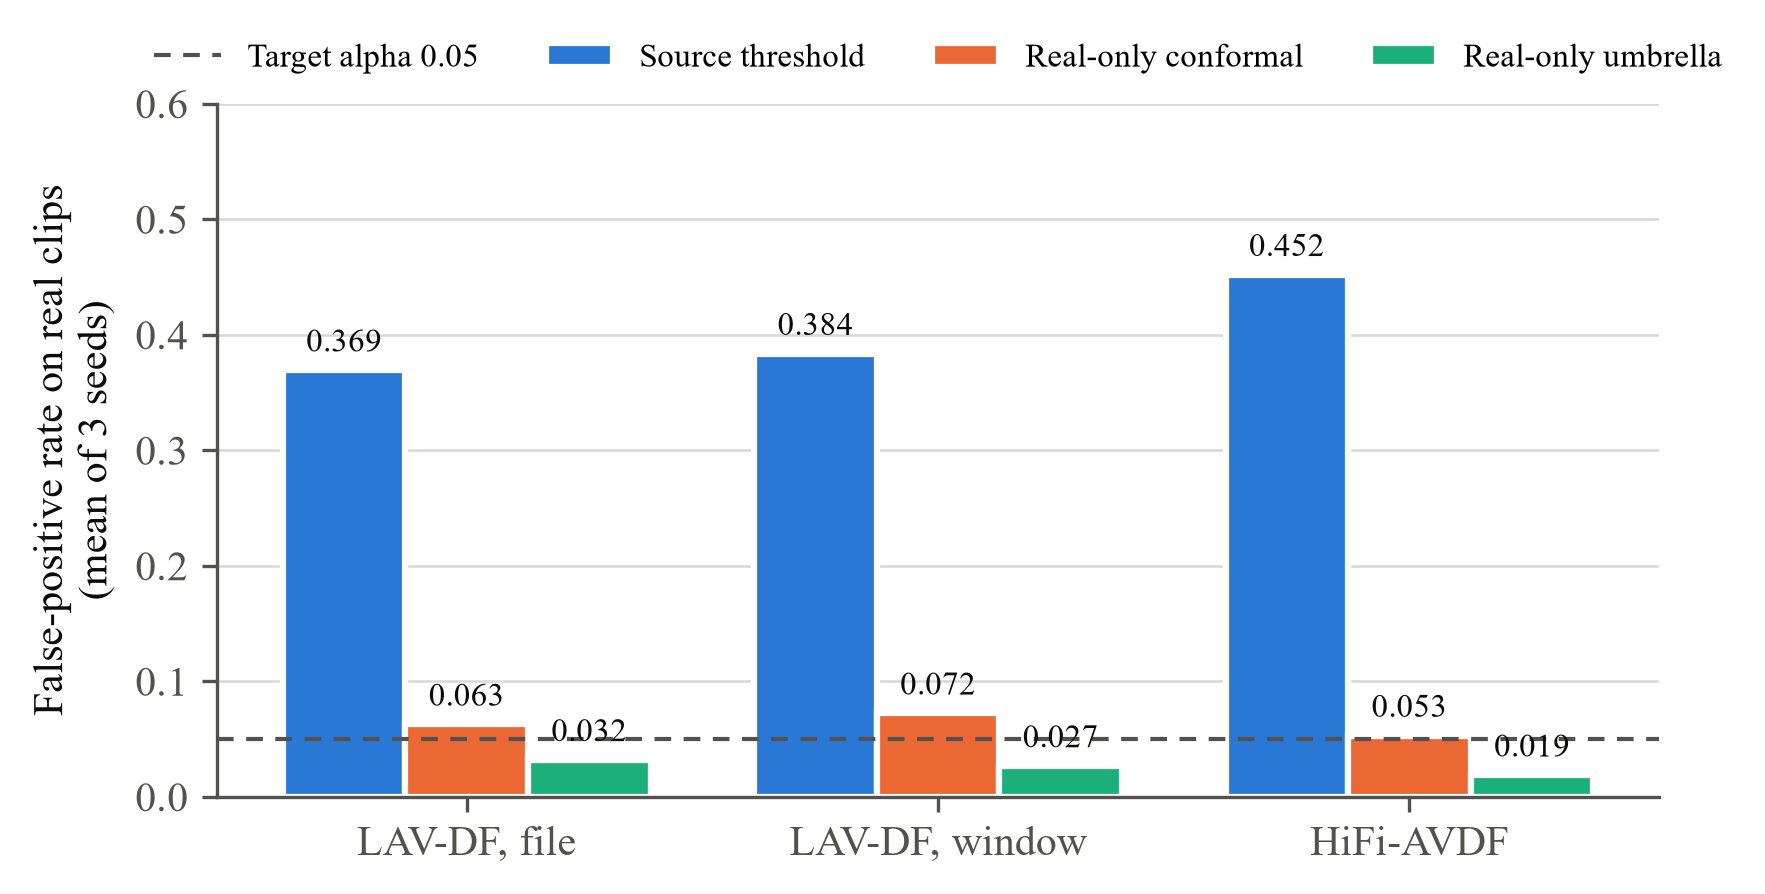
\includegraphics[width=\columnwidth]{fig_h4.png}}
\caption{Realized FPR and TPR of the three threshold rules on each H4 target
and seed (Table~\ref{tab:h4}).}
\label{fig:h4}
\end{figure}

\section{Fusion Against Visual-Only (H2)}
\label{sec:h2}

\subsection{Visual and audio paths}

The visual path is EfficientNet-B0 with a GRU over face frames, trained on the
video label. The audio path is Wav2Vec2 Base with attentive pooling, trained
on the audio label. Both train on the neutral FakeAVCeleb training partition,
thinned to three video-fake clips per real-video clip, at seeds 17, 29 and 43.
Each picks its epoch and threshold on validation.

\begin{table}[htbp]
\caption{Visual and audio paths on the identity-strict neutral FakeAVCeleb
test (ROC-AUC, 95\% identity-bootstrap interval), each on its own label}
\label{tab:branches}
\centering
\begin{tabular}{lrr}
\toprule
Seed & Visual (video label) & Audio (audio label) \\
\midrule
17 & {{visual.test-identity-strict.seed17.auc}} [{{visual.test-identity-strict.seed17.auc_low}}, {{visual.test-identity-strict.seed17.auc_high}}] & {{audio.test-identity-strict.seed17.auc}} [{{audio.test-identity-strict.seed17.auc_low}}, {{audio.test-identity-strict.seed17.auc_high}}] \\
29 & {{visual.test-identity-strict.seed29.auc}} [{{visual.test-identity-strict.seed29.auc_low}}, {{visual.test-identity-strict.seed29.auc_high}}] & {{audio.test-identity-strict.seed29.auc}} [{{audio.test-identity-strict.seed29.auc_low}}, {{audio.test-identity-strict.seed29.auc_high}}] \\
43 & {{visual.test-identity-strict.seed43.auc}} [{{visual.test-identity-strict.seed43.auc_low}}, {{visual.test-identity-strict.seed43.auc_high}}] & {{audio.test-identity-strict.seed43.auc}} [{{audio.test-identity-strict.seed43.auc_low}}, {{audio.test-identity-strict.seed43.auc_high}}] \\
\bottomrule
\end{tabular}
\end{table}

\subsection{Fusion and test}

The fusion was fixed in a dated amendment before any visual or audio model
existed. It is a logistic regression on the three standardized branch logits,
fit on FakeAVCeleb validation. Training clips are excluded because each branch
was fit on them. The fusion's own validation scores, which set its threshold,
come from 5-fold cross-fitting grouped by identity. The model applied to test
and to the targets is refit on all of validation. A clip counts only if all
three paths score it, and the visual path is compared on exactly those clips.

The label is the clip label: a clip is fake if either stream is fake. The
statistic is AUC(fusion) minus AUC(visual), averaged over the three seeds. Its
interval comes from 1,000 bootstrap resamples of identities, shared by all
seeds. The one-sided $p$-value is the share of resamples at or below zero.
Holm correction at 0.05 runs over three targets: DFDC, LAV-DF test and the
identity-strict FakeAVCeleb test. H2 holds if at least two survive.

\begin{table*}[htbp]
\caption{H2: fusion minus visual-only ROC-AUC per seed, and the mean of three
seeds with a 95\% identity-bootstrap interval; Holm at 0.05 over the first
three rows}
\label{tab:h2}
\centering
\begin{tabular}{lrrrrrrl}
\toprule
Target & Clips & Seed 17 & Seed 29 & Seed 43 & Mean [95\%] & $p$ & Holm \\
\midrule
FakeAVCeleb test, strict & {{h2.test-identity-strict.clips|int}} & {{h2.test-identity-strict.seed17}} & {{h2.test-identity-strict.seed29}} & {{h2.test-identity-strict.seed43}} & {{h2.test-identity-strict.estimate}} [{{h2.test-identity-strict.lower}}, {{h2.test-identity-strict.upper}}] & {{h2.test-identity-strict.p|p}} & {{h2.test-identity-strict.holm}} \\
DFDC & {{h2.dfdc.clips|int}} & {{h2.dfdc.seed17}} & {{h2.dfdc.seed29}} & {{h2.dfdc.seed43}} & {{h2.dfdc.estimate}} [{{h2.dfdc.lower}}, {{h2.dfdc.upper}}] & {{h2.dfdc.p|p}} & {{h2.dfdc.holm}} \\
LAV-DF test, window & {{h2.lavdf-window.clips|int}} & {{h2.lavdf-window.seed17}} & {{h2.lavdf-window.seed29}} & {{h2.lavdf-window.seed43}} & {{h2.lavdf-window.estimate}} [{{h2.lavdf-window.lower}}, {{h2.lavdf-window.upper}}] & {{h2.lavdf-window.p|p}} & {{h2.lavdf-window.holm}} \\
\midrule
HiFi-AVDF (reported) & {{h2.hifiavdf.clips|int}} & {{h2.hifiavdf.seed17}} & {{h2.hifiavdf.seed29}} & {{h2.hifiavdf.seed43}} & {{h2.hifiavdf.estimate}} [{{h2.hifiavdf.lower}}, {{h2.hifiavdf.upper}}] & {{h2.hifiavdf.p|p}} & n/a \\
\bottomrule
\end{tabular}
\end{table*}

\begin{figure}[htbp]
\centerline{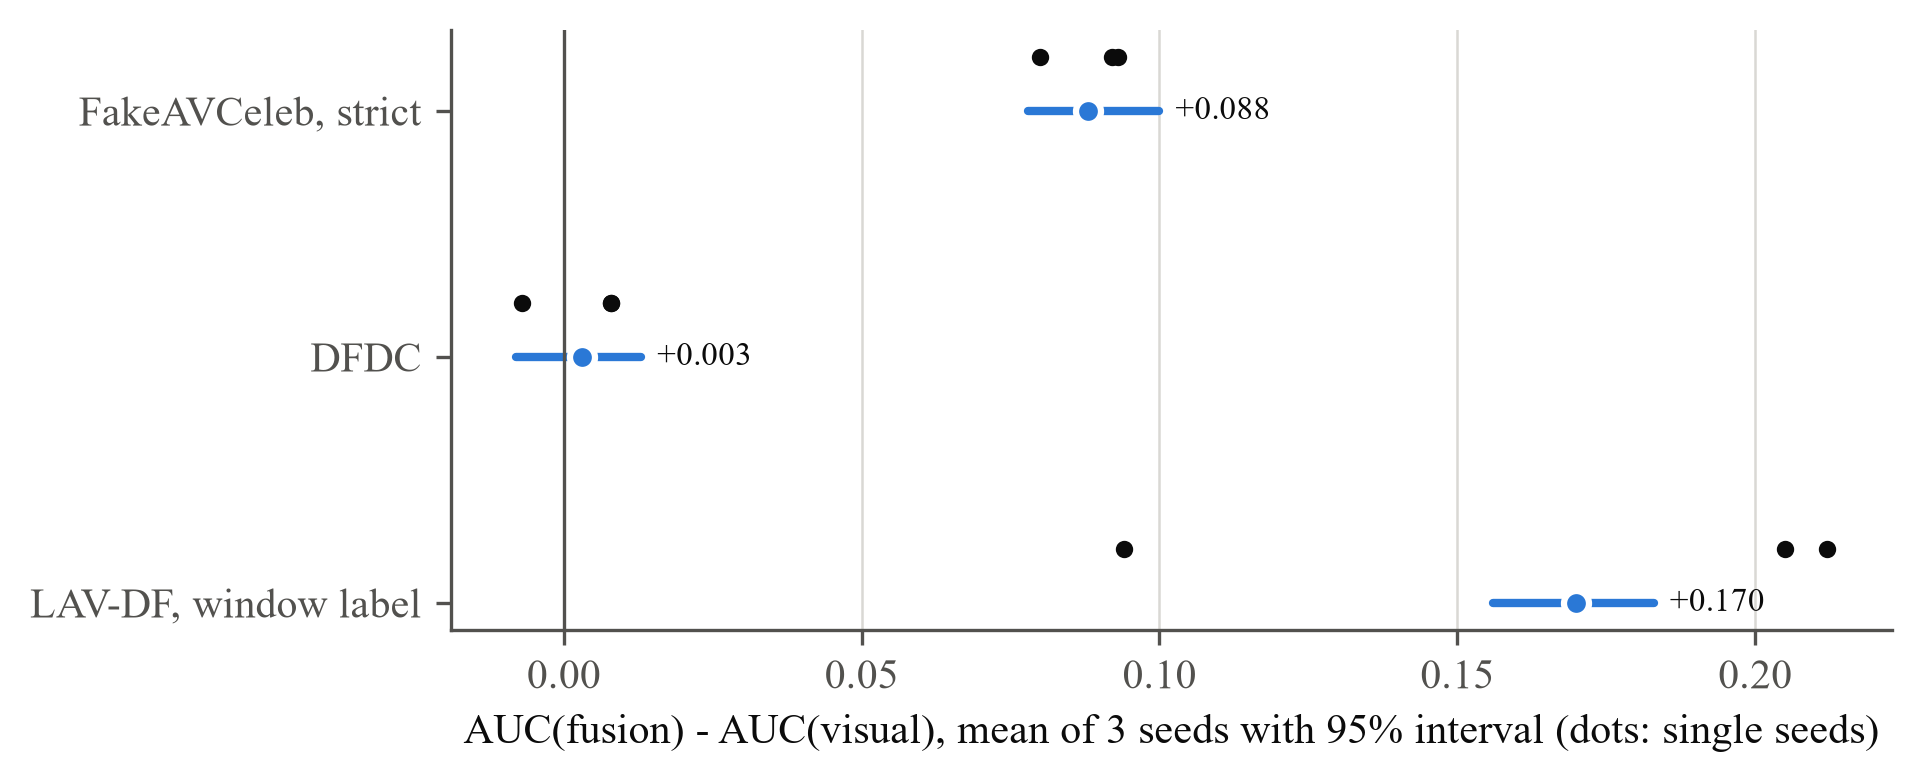
\includegraphics[width=\columnwidth]{fig_h2.png}}
\caption{Fusion minus visual-only ROC-AUC per target: the mean of three seeds
with its 95\% identity-bootstrap interval, and each seed as a dot
(Table~\ref{tab:h2}).}
\label{fig:h2}
\end{figure}

Table~\ref{tab:h2} and Fig.~\ref{fig:h2} give the result. FakeAVCeleb and
LAV-DF survive Holm correction and DFDC does not, so H2 holds by its
preregistered rule. The seed-17 fusion weights on the standardized logits
are {{h2.weights.seed17.visual}} (visual), {{h2.weights.seed17.audio}} (audio)
and {{h2.weights.seed17.sync}} (sync).

\begin{table}[htbp]
\caption{ROC-AUC of each path on the clip label, over the clips H2 compares:
lowest and highest of three seeds}
\label{tab:h2levels}
\centering
\small
\begin{tabular}{lllll}
\toprule
Target & Visual & Audio & Sync & Fusion \\
\midrule
FakeAVCeleb, strict & {{h2.test-identity-strict.auc.visual.min}}, {{h2.test-identity-strict.auc.visual.max}} & {{h2.test-identity-strict.auc.audio.min}}, {{h2.test-identity-strict.auc.audio.max}} & {{h2.test-identity-strict.auc.sync.min}}, {{h2.test-identity-strict.auc.sync.max}} & {{h2.test-identity-strict.auc.fusion.min}}, {{h2.test-identity-strict.auc.fusion.max}} \\
DFDC & {{h2.dfdc.auc.visual.min}}, {{h2.dfdc.auc.visual.max}} & {{h2.dfdc.auc.audio.min}}, {{h2.dfdc.auc.audio.max}} & {{h2.dfdc.auc.sync.min}}, {{h2.dfdc.auc.sync.max}} & {{h2.dfdc.auc.fusion.min}}, {{h2.dfdc.auc.fusion.max}} \\
LAV-DF, window & {{h2.lavdf-window.auc.visual.min}}, {{h2.lavdf-window.auc.visual.max}} & {{h2.lavdf-window.auc.audio.min}}, {{h2.lavdf-window.auc.audio.max}} & {{h2.lavdf-window.auc.sync.min}}, {{h2.lavdf-window.auc.sync.max}} & {{h2.lavdf-window.auc.fusion.min}}, {{h2.lavdf-window.auc.fusion.max}} \\
\midrule
HiFi-AVDF (reported) & {{h2.hifiavdf.auc.visual.min}}, {{h2.hifiavdf.auc.visual.max}} & {{h2.hifiavdf.auc.audio.min}}, {{h2.hifiavdf.auc.audio.max}} & {{h2.hifiavdf.auc.sync.min}}, {{h2.hifiavdf.auc.sync.max}} & {{h2.hifiavdf.auc.fusion.min}}, {{h2.hifiavdf.auc.fusion.max}} \\
\bottomrule
\end{tabular}
\end{table}

The result is weaker than the verdict suggests.
Two checks, run after the verdict and so exploratory, find that no target
shows fusion improving on fakes the visual path can see
(Table~\ref{tab:h2levels}).

On the FakeAVCeleb test the whole gain comes from the cloned-voice clips.
They have real video, and the visual path was trained never to flag them.
Without them, the gain falls from {{h2.test-identity-strict.estimate}} to
between {{h2.test-identity-strict.without_cloned_voice.min}} and
{{h2.test-identity-strict.without_cloned_voice.max}} per seed.

On LAV-DF the visual path ranks every fake type below the original real files
(AUC {{visual.lavdf-test.type.min}} to {{visual.lavdf-test.type.max}}). That
includes clips whose video was never edited
({{visual.lavdf-test.type.RealVideo-FakeAudio.min}} to
{{visual.lavdf-test.type.RealVideo-FakeAudio.max}}). So it reacts to some
difference between LAV-DF's real and fake files that is not the face edit,
and reads it backwards. What that difference is, we do not know. The file-cue
audit reads metadata and cannot see it, and six frame statistics (sharpness,
high frequencies, blockiness, brightness, contrast, motion; amendment A13,
exploratory) do not explain it either: each separates the two groups at AUC
{{a13.lavdf.auc_min}} to {{a13.lavdf.auc_max}}, all six together at
{{a13.lavdf.all_six}}, against the path's {{a13.lavdf.visual}}. Its pooled AUC
in Table~\ref{tab:h2levels} is higher, though still below chance, because the
window label counts as real the clips cut from fake files with no edit in the
window, and the path scores those as low as the fakes. Fusion beats this
reversed baseline but trails the audio and sync paths alone in every seed.
Section~\ref{sec:a12} tests whether its FakeAVCeleb weights are to blame.

On DFDC, the one target where the visual path is fair, every clip in our
subset has real audio and fusion adds nothing. HiFi-AVDF, reported outside the
rule, repeats the LAV-DF pattern: fusion gains {{h2.hifiavdf.estimate}} over a
visual path near chance but trails the audio path alone in every seed. The
weights also vary by seed: the audio weight is {{h2.weights.seed17.audio}},
{{h2.weights.seed29.audio}} and {{h2.weights.seed43.audio}} for seeds 17, 29
and 43.

So H2 shows that an audio path catches audio fakes a visual path cannot. It
does not show that fusion improves detection, or that it transfers to a new
corpus.

\subsection{Exploratory: a fusion fit on other corpora (A12)}
\label{sec:a12}

Amendment A12, fixed after H2 was read, refits the same fusion in two ways
from the same logits. The \textit{leave-one-out} fusion is fit on the other two
targets and never sees the one it scores. The \textit{upper bound} is a
5-fold cross-fit by identity on the target itself. It uses the target's labels,
so it is not a detector; it shows whether the three paths hold any
complementary information there (Table~\ref{tab:a12}).

\begin{table*}[htbp]
\caption{A12 (exploratory): ROC-AUC on the clip label, mean of three seeds}
\label{tab:a12}
\centering
\begin{tabular}{lrrrrrr}
\toprule
Target & Visual & Audio & Sync & A8 fusion & Leave one out & Upper bound \\
\midrule
DFDC & {{a12.dfdc.auc.visual}} & {{a12.dfdc.auc.audio}} & {{a12.dfdc.auc.sync}} & {{a12.dfdc.auc.a8}} & {{a12.dfdc.auc.leave_one_out}} & {{a12.dfdc.auc.upper_bound}} \\
LAV-DF, window & {{a12.lavdf-window.auc.visual}} & {{a12.lavdf-window.auc.audio}} & {{a12.lavdf-window.auc.sync}} & {{a12.lavdf-window.auc.a8}} & {{a12.lavdf-window.auc.leave_one_out}} & {{a12.lavdf-window.auc.upper_bound}} \\
HiFi-AVDF & {{a12.hifiavdf.auc.visual}} & {{a12.hifiavdf.auc.audio}} & {{a12.hifiavdf.auc.sync}} & {{a12.hifiavdf.auc.a8}} & {{a12.hifiavdf.auc.leave_one_out}} & {{a12.hifiavdf.auc.upper_bound}} \\
\bottomrule
\end{tabular}
\end{table*}

On DFDC and HiFi-AVDF even the upper bound does not beat the best single
path: {{a12.dfdc.upper_bound-minus-visual.estimate}}
[{{a12.dfdc.upper_bound-minus-visual.lower}},
{{a12.dfdc.upper_bound-minus-visual.upper}}] over the visual path on DFDC, and
{{a12.hifiavdf.upper_bound-minus-audio.estimate}}
[{{a12.hifiavdf.upper_bound-minus-audio.lower}},
{{a12.hifiavdf.upper_bound-minus-audio.upper}}] over the audio path on
HiFi-AVDF. There, no weighting of these paths helps. On LAV-DF the upper bound
beats the audio path by {{a12.lavdf-window.upper_bound-minus-audio.estimate}},
and the leave-one-out fusion beats the A8 fusion by
{{a12.lavdf-window.leave_one_out-minus-a8.estimate}}, but it still trails the
audio path ({{a12.lavdf-window.leave_one_out-minus-audio.estimate}}). The best
path changes with the corpus: visual on DFDC, audio on the other two. So weights
fit on some corpora point the wrong way on the next, and on DFDC the
leave-one-out fusion falls to {{a12.dfdc.auc.leave_one_out}}, below chance.
The FakeAVCeleb weights explain part of the LAV-DF loss, but the larger problem
is that no fixed fusion of these paths transfers between these corpora.

\section{Exploratory: Stronger Frozen Backbones (A11)}
\label{sec:a11}

Published work reports that frozen CLIP ViT-L/14 features transfer far better
for faces, and XLS-R far better for speech, than the backbones P-001 uses. That
evidence comes from raw files. Amendment A11, fixed before either model
existed, trains both frozen on the same cleaned data, splits and seeds, and
compares each with its P-001 path on the same clips
(Table~\ref{tab:a11}).

\begin{table}[htbp]
\caption{A11 (exploratory): new path minus P-001 path, ROC-AUC on each path's
own label, mean of three seeds with a 95\% identity-bootstrap interval}
\label{tab:a11}
\centering
\small
\begin{tabular}{lll}
\toprule
Set & CLIP $-$ visual & XLS-R $-$ audio \\
\midrule
FakeAVCeleb, strict & {{a11.clip-vs-visual.test-identity-strict.estimate}} [{{a11.clip-vs-visual.test-identity-strict.lower}}, {{a11.clip-vs-visual.test-identity-strict.upper}}] & {{a11.xlsr-vs-audio.test-identity-strict.estimate}} [{{a11.xlsr-vs-audio.test-identity-strict.lower}}, {{a11.xlsr-vs-audio.test-identity-strict.upper}}] \\
DFDC & {{a11.clip-vs-visual.dfdc.estimate}} [{{a11.clip-vs-visual.dfdc.lower}}, {{a11.clip-vs-visual.dfdc.upper}}] & one class \\
LAV-DF test & {{a11.clip-vs-visual.lavdf-test.estimate}} [{{a11.clip-vs-visual.lavdf-test.lower}}, {{a11.clip-vs-visual.lavdf-test.upper}}] & {{a11.xlsr-vs-audio.lavdf-test.estimate}} [{{a11.xlsr-vs-audio.lavdf-test.lower}}, {{a11.xlsr-vs-audio.lavdf-test.upper}}] \\
HiFi-AVDF & {{a11.clip-vs-visual.hifiavdf.estimate}} [{{a11.clip-vs-visual.hifiavdf.lower}}, {{a11.clip-vs-visual.hifiavdf.upper}}] & {{a11.xlsr-vs-audio.hifiavdf.estimate}} [{{a11.xlsr-vs-audio.hifiavdf.lower}}, {{a11.xlsr-vs-audio.hifiavdf.upper}}] \\
\bottomrule
\end{tabular}
\end{table}

On cleaned data neither backbone transfers better. XLS-R matches the P-001
audio path in-domain and is worse on LAV-DF and HiFi-AVDF. On HiFi-AVDF it
reaches {{a11.xlsr-vs-audio.hifiavdf.auc_new}} against
{{a11.xlsr-vs-audio.hifiavdf.auc_old}}.
CLIP falls to {{a11.clip-vs-visual.test-identity-strict.auc_new}} in-domain
and to {{a11.clip-vs-visual.hifiavdf.auc_new}} on HiFi-AVDF. Its one gain, on
LAV-DF, takes it to {{a11.clip-vs-visual.lavdf-test.auc_new}}: near chance,
where the P-001 visual path is inverted
({{a11.clip-vs-visual.lavdf-test.auc_old}}). CLIP does not read the difference
between LAV-DF's real and fake files that inverts the P-001 path, but it does
not detect LAV-DF's fakes either. Our recipe differs from the published ones (no
LayerNorm tuning for CLIP, no weighted sum of XLS-R layers), so a published
recipe might do better. Under ours, the advantage measured on raw files does
not survive the shortcut control.

\section{Exploratory: Five Gaps Checked (A15 to A19)}
\label{sec:overnight}

Five more checks were fixed as dated amendments before their results existed.
None changes a verdict.

\textit{The sync mechanism (A16).} On all {{a16.clips}} real FakeAVCeleb test
clips we kept the lips and moved the audio. Against the original window, the
misfit separates audio moved by one frame at AUC {{a16.shift004.auc}}
[{{a16.shift004.low}}, {{a16.shift004.high}}], by 0.2~s at {{a16.shift020.auc}},
and another person's audio at {{a16.swap.auc}}. Shifts of one and two frames
are smaller than any the head saw in training. The test does not cover cloned
voices, which are new audio rather than moved audio.

\textit{Which stream was faked, one direction (A15).} The visual and audio
paths act as video-fake and audio-fake heads on LAV-DF, at their FakeAVCeleb
thresholds. Their macro-F1 is {{a15.window.heads.min}} to
{{a15.window.heads.max}}, against {{a15.window.baseline}} for a predictor that
marks both streams fake whenever the clip is fake: a difference of
{{a15.window.estimate}} [{{a15.window.lower}}, {{a15.window.upper}}]. The video
head's precision ({{a15.window.video.seed17.precision}} at seed 17) is below
the share of edited videos. The audio head is precise but, at its source
threshold, recalls {{a15.window.audio.seed43.recall}} to
{{a15.window.audio.seed17.recall}} of audio fakes at seeds 43 and 17. The
reverse direction needs models trained on LAV-DF, so H3 has still not run.

\textit{Speaker overlap (A17).} All {{a17.sources.dev}} FakeAVCeleb source
identities are VoxCeleb2 dev speakers, and none are test speakers. AV-HuBERT
pretrained on the English part of VoxCeleb2 dev, so every FakeAVCeleb speaker
may have been heard by the frozen encoder. No unseen speaker exists in this
corpus to measure the effect.

\textit{H1 with a fixed bitrate (A18).} Video bitrate was the leading cue left
after cleaning. Re-encoding all of FakeAVCeleb at a constant 160~kb/s instead of
a constant quality lowers the clip-label ceiling only from
{{audit.fakeavceleb.neutral.clip}} to {{audit.fakeavceleb.cbr.clip}}, still
above 0.60. The encoder overshoots its target slightly on busier content, and
the overshoot still follows the label; trailing silence and loudness remain.

\textit{A published method on our protocol (A19).} We retrained AVH-Align's
head, loss and score~\cite{smeu2025} on our real training windows and frozen
features. It does not beat our sync path on any set. It is worse on the
identity-strict test ({{a19.test-identity-strict.minus_sync.estimate}}
[{{a19.test-identity-strict.minus_sync.lower}},
{{a19.test-identity-strict.minus_sync.upper}}]), DFDC
({{a19.dfdc.minus_sync.estimate}}) and HiFi-AVDF
({{a19.hifiavdf.minus_sync.estimate}}), narrowly worse on LAV-DF under the
file label ({{a19.lavdf-test.minus_sync.estimate}}), and level under the window
label ({{a19.lavdf-window.minus_sync.estimate}}) and on the full test set. On DFDC and HiFi-AVDF it
scores {{a19.dfdc.auc}} and {{a19.hifiavdf.auc}}. The published system, with
fine-tuned AV-HuBERT Large features, was not run: that checkpoint is not
available to us.

\section{Limitations}

\textit{H1 missed its bar.} The neutral FakeAVCeleb ceiling is
{{audit.fakeavceleb.neutral.clip}} against a preregistered 0.60. Video
bitrate remains as a cue. It follows image content under constant-quality
encoding, but the test was defined on all cues, and it failed. A fixed bitrate
does not fix it either (A18).

\textit{A residual audio cue remains.} The audio-label ceiling on the neutral
copies is {{audit.fakeavceleb.neutral.audio}}. It comes from small edge
differences and from loudness after AAC encoding. It weakens any claim about
audio, including part of the voice-cloning row in Table~\ref{tab:methods}.
The audio path does not rely on those two cues, though. With loudness levelled
and 250~ms cut from each edge (amendment A14, exploratory), its
identity-strict AUC stays between {{a14.test-identity-strict.perturbed_min}}
and {{a14.test-identity-strict.perturbed_max}}. Cues the audit did not name are
not covered.

\textit{Cleaning refuses clips.} The {{neutral.fakeavceleb.refused|int}}
refused clips are all generated speech, so the neutral data are not a random
subset of the raw data.

\textit{Few baselines.} H3 has run in one direction only (A15). The
StreamFusion model, our secondary fusion, was not run. AVH-Align's method ran
on our protocol (A19), but not its published system, and HAVIC has not been
run.

\textit{One training corpus.} Every model learns from FakeAVCeleb alone: about
500 real videos from 2021, with crude fakes, and about 350 speakers for the
sync path. The cross-corpus results show how a detector trained this way
transfers once the shortcuts are gone, not that every detector fails. Training
on several corpora with one held out at a time would test whether more variety
helps.

\textit{Speaker overlap.} Every FakeAVCeleb speaker is in VoxCeleb2 dev,
which AV-HuBERT pretrained on (A17). LAV-DF is also built from VoxCeleb2 but
has no speaker ids. Some signal may come from the encoder having heard a
speaker before; with no unseen speaker in FakeAVCeleb, we cannot measure how
much.

\textit{DFDC is too small for H4.} Our DFDC subset has
{{audit.dfdc.raw.census.RealVideo-RealAudio.clips|int}} real clips, fewer than
the 200 needed for calibration, so H4 covers two targets only.

\section{Conclusion}

Audio-visual deepfake benchmarks leak their labels through their files. On
FakeAVCeleb and HiFi-AVDF, file metadata and audio edges alone come close to
perfect separation. Codec, audio format, clip length, frame size and edge
silence each tell a classifier which pipeline made the clip. A detector score
on these corpora means little until it is set beside that ceiling.

Our first neutralizer re-introduced leading silence through AAC priming. The
final version lowers the FakeAVCeleb ceiling to
{{audit.fakeavceleb.neutral.clip}}, which still misses our preregistered bar.
We report the residual and the clips it removes.

A lip-sync detector trained only on real clips scores above that ceiling on
the neutral copies, and its per-method scores follow what each method does to
the lips and the voice. On corpora it never saw it stays above chance but falls
far (Section~\ref{sec:cross}). A threshold set from real clips of the new
corpus keeps false alarms near the target, at the cost of recall.

Fusing the three paths passes its preregistered test, but only through fakes
the visual path cannot see or a visual path that the LAV-DF files invert. No
fixed fusion of these paths transferred between corpora (A12), and stronger
frozen backbones did not transfer better on cleaned data (A11). We suggest
that every audio-visual benchmark result be reported beside a shortcut
ceiling, and with the clips that cleaning removed.

\section*{Acknowledgment}

Claude (Anthropic) assisted with implementation, analysis and documentation.
All design decisions, results and claims were reviewed by the authors.

\begin{thebibliography}{00}
\bibitem{fakeavceleb} H. Khalid, S. Tariq, M. Kim, and S. S. Woo,
``FakeAVCeleb: A novel audio-video multimodal deepfake dataset,'' in
\textit{Proc. NeurIPS Datasets and Benchmarks Track}, 2021.
\bibitem{lavdf} Z. Cai, K. Stefanov, A. Dhall, and M. Hayat, ``Do you really
mean that? Content driven audio-visual deepfake dataset and multimodal method
for temporal forgery localization,'' in \textit{Proc. DICTA}, 2022.
\bibitem{dfdc} B. Dolhansky, J. Bitton, B. Pflaum, J. Lu, R. Howes, M. Wang,
and C. Canton Ferrer, ``The DeepFake Detection Challenge (DFDC) dataset,''
arXiv:2006.07397, 2020.
\bibitem{havic} J. Peng, Y. Wang, Y. Li, L. Kong, and X. Hong, ``Leave no
stone unturned: Uncovering holistic audio-visual intrinsic coherence for
deepfake detection,'' in \textit{Proc. CVPR Findings}, 2026, arXiv:2603.23960.
\bibitem{avhubert} B. Shi, W.-N. Hsu, K. Lakhotia, and A. Mohamed, ``Learning
audio-visual speech representation by masked multimodal cluster prediction,''
in \textit{Proc. ICLR}, 2022.
\bibitem{avff} T. Oorloff, S. Koppisetti, N. Bonettini, D. Solanki,
B. Colman, Y. Yacoob, A. Shahriyari, and G. Bharaj, ``AVFF: Audio-visual
feature fusion for video deepfake detection,'' in \textit{Proc. CVPR}, 2024.
\bibitem{smeu2025} S. Smeu, D.-A. Boldisor, D. Oneata, and E. Oneata,
``Circumventing shortcuts in audio-visual deepfake detection datasets with
unsupervised learning,'' in \textit{Proc. CVPR}, 2025, arXiv:2412.00175.
\bibitem{muller2021} N. M. M\"uller, F. Dieckmann, P. Czempin, R. Canals,
K. B\"ottinger, and J. Williams, ``Speech is silver, silence is golden: What do
ASVspoof-trained models really learn?'' in \textit{Proc. ASVspoof 2021
Workshop}, 2021.
\bibitem{deepfakedoctor} M. Klemt, C. Segna, and A. Rohrbach, ``DeepFake
Doctor: Diagnosing and treating audio-video fake detection,''
arXiv:2506.05851, 2025.
\bibitem{pagon2026} S. Pagon, Y. Shen, V. Asnani, and F. Liu, ``What do
deepfake benchmarks measure? An audit using frozen self-supervised
representations,'' arXiv:2606.26384, 2026.
\bibitem{dfdlab2026} J. Rybarczyk, M. Roszkowski, and J. Komorowski,
``DFD-Lab: A modular audio-visual deepfake detection pipeline,''
arXiv:2609.23830, 2026.
\bibitem{grommelt} P. Grommelt \textit{et al.}, ``Fake or JPEG? Revealing
common biases in generated image detection datasets,'' arXiv:2403.17608,
2024.
\bibitem{multimodaltrace} M. A. Raza and K. M. Malik, ``Multimodaltrace:
Deepfake detection using audiovisual representation learning,'' in
\textit{Proc. CVPR Workshops}, 2023.
\bibitem{yu2023} C. Yu \textit{et al.}, ``A unified framework for
modality-agnostic deepfakes detection,'' arXiv:2307.14491, 2023; published as
``Modality-agnostic deepfakes detection'' in \textit{Proc. ACM IH\&MMSec},
2025.
\bibitem{mrdf} H. Zou, M. Shen, Y. Hu, C. Chen, E. S. Chng, and D. Rajan,
``Cross-modality and within-modality regularization for audio-visual
deepfake detection,'' in \textit{Proc. ICASSP}, 2024.
\bibitem{bates2023} S. Bates, E. Cand\`es, L. Lei, Y. Romano, and M. Sesia,
``Testing for outliers with conformal p-values,'' \textit{Annals of
Statistics}, vol. 51, no. 1, 2023.
\bibitem{tong2018} X. Tong, Y. Feng, and J. J. Li, ``Neyman-Pearson
classification algorithms and NP receiver operating characteristics,''
\textit{Science Advances}, vol. 4, no. 2, 2018.
\bibitem{nguyen2026} D. Nguyen \textit{et al.}, ``When AUC misleads:
Polarization-aware evaluation of deepfake detectors under domain shift,''
arXiv:2606.19184, 2026.
\bibitem{laionmobile} A. von Stryk and J. Keuper, ``LAION-Mobile: Evaluating
deepfake detectors on one million smartphone photos,'' arXiv:2609.11134,
2026.
\bibitem{mahdaoui2026} M. Mahdaoui, ``How many real photos does it take?
Finite-sample false-alarm control of frozen AI-image detectors under paired
camera-processing shift (preregistration v1.0),'' Zenodo, record 23863746,
2026.
\bibitem{pgag2026} S. Alqaraleh, ``PGA-G: Selective adaptation and conformal
calibration for speech deepfake detection,'' Zenodo, record 23652611, 2026.
\end{thebibliography}

\end{document}
